%!TEX root = ../main.tex
% !TeX spellcheck = en_GB 
\chapter{Evaluation}%----------------------------------------------------------------
%------------------------------------------------------------------------------------


\label{sec:evaluation}
Five scenarios are defined in order to test the ANS in multi vessel situations. However, a simple crossing scenario is first shown to test the algorithm in a basic COLREGs situation. Ideas for the other scenarios are from \textcite{ecolreg_overtaking-and-crossing-2,ecolreg_overtaking-and-crossing-3,ecolreg_overtaking-and-crossing,ecolreg_overtaking-and-head-on}, with a few minor modifications. All scenarios are set in high visibility on the high sea.



\section{Crossing scenario}%---------------------------------------------------------
%------------------------------------------------------------------------------------


\begin{figure}[H]
    \centering
    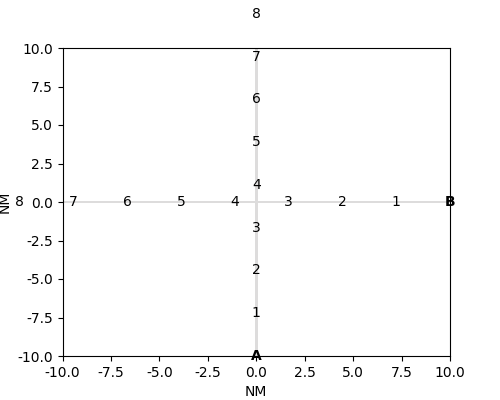
\includegraphics[width=0.75\textwidth,height=0.75\textheight,keepaspectratio]{../src/img/crossing.png}
    \caption{Crossing scenario}
    \label{fig:simple-scen}
\end{figure}

The first scenario depicts a simple crossing situation where two vessels are on perpendicular courses. The vessels start  approximately 14 NM from each other with a speed of 10 kts as seen in figure \ref{fig:simple-scen}. The vessels maximum speed is set to 12 kts and maximum rate of turn \ang{3} per second. The two vessels are to  collide in origo if no corrections are made to either course or speed. COLREGs \textit{rule 15} stipulate that vessel (\textit{A}) that has the other vessel on its starboard side  in a crossing situation should alter its course to starboard, thereby, avoiding passing in front of the other vessel (\textit{B}).
\begin{figure}[H]
    \centering
    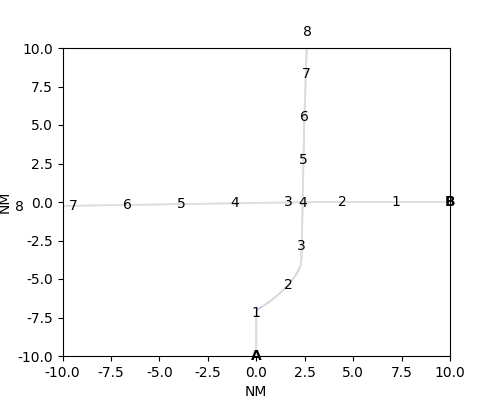
\includegraphics[width=0.75\textwidth,height=0.75\textheight,keepaspectratio]{../src/img/crossing_res.png}
    \caption{Crossing scenario}
    \label{fig:simple-scen-res}
\end{figure}

Figure \ref{fig:simple-scen-res} shows the scenario when both boats are guided by the FIS system. The numbers on the vessels tracks are printed every thousand seconds, which equal 16 minutes and 40 seconds, and help to compare the vessels positions at  given time frames. These numbers will from here on be referred to with bold numbers.

It can be seen that both vessels continue along their original paths until vessel \textit{A} reaches \textbf{1}, at which point the distance to vessel \textit{B} has shrunk to 10 NM and the algorithm becomes aware of the target vessel. Vessel \textit{A} will at this point initiate a starboard turn  of \ang{24}  to pass behind vessel \textit{B} as specified in COLREGs. Vessel \textit{A} will then follow headings suggested by the ANS until \textbf{2.7} where  vessel \textit{B} is no longer considered a threat, i.e. no rule in the FIS applies, after which it steers back to its original heading. Vessel \textit{B} will during the whole scenario be the stand on vessel and, therefore, keep its course and speed.

The ANS suggestions are exactly as described in the COLREGS documents for this case. The manoeuvre is initiated at a distance of 10 NM, which can be regarded as ample time (\textit{Rule 8}). The correction is, furthermore, large and therefore clearly visible to the other vessels involved.

\section{Overtaking and head-on scenario}%-------------------------------------------
%------------------------------------------------------------------------------------


\begin{figure}[H]
    \centering
    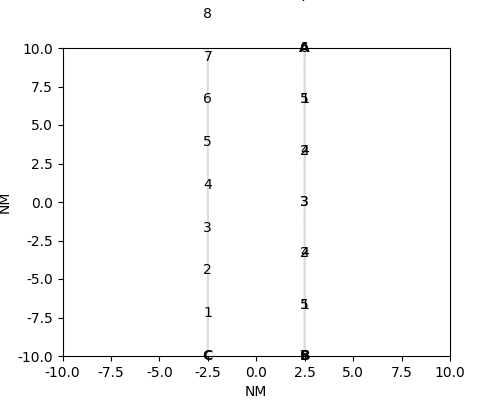
\includegraphics[width=0.75\textwidth,height=0.75\textheight,keepaspectratio]{../src/img/overtaking_head_on.png}
    \caption[Overtaking and head-on scenario]{Overtaking and head-on scenario  \cite{ecolreg_overtaking-and-head-on}}
    \label{fig:overtaking-and-head-on}
\end{figure}
This scenario defines a three vessel scenario, where two vessels are meeting on  reciprocal courses. One of the vessels is, furthermore, overtaking a third vessel on the stand on vessels starboard side. A visualization of the scenario is shown in figure \ref{fig:overtaking-and-head-on}. Vessels \textit{A} and \textit{B} starts on reciprocal tracks 20 NM from each other, while \textit{B} and \textit{C} start abreast 5 NM from each other. \textit{A}, \textit{B}, and \textit{C} has a maximum speed of 15 kts. \textit{A} and \textit{B} start at 12 kts while \textit{C} is slightly slower at 10 kts. Maximum rate of turn of all vessels is set to \ang{3} per second.

Vessels \textit{A} and \textit{B} are obliged to alter their courses to starboard to prevent a head-on collision (\textit{Rule 14}). Moreover, vessel \textit{B} shall keep out of the way of \textit{C}  and in no circumstance alter its course so that it becomes a crossing vessel to \textit{C} (\textit{Rule 13}). All corrections shall furthermore be ample, so that it is recognizable by the other vessel, and taken as early as possible (\textit{Rule 16}) \cite{ecolreg_overtaking-and-head-on}.

\textcite{ecolreg_overtaking-and-head-on} suggest that vessel \textit{A} should alter course to starboard and pass ahead of vessel C,  to avoid a collision.



\begin{figure}[H]
    \centering
    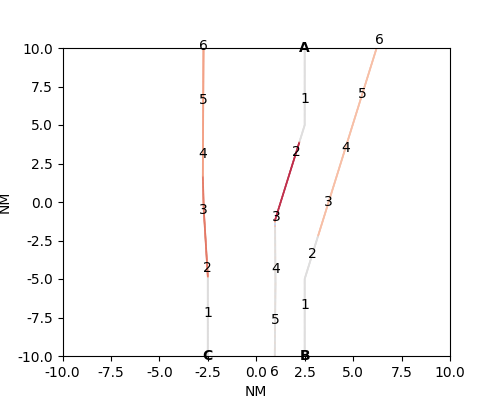
\includegraphics[width=0.75\textwidth,height=0.75\textheight,keepaspectratio]{../src/img/overtaking_head_on_res.png}
    \caption{Overtaking and head-on scenario  }
    \label{fig:overtaking-and-head-on-res}
\end{figure}
The same initial scenario with the ANS enabled can be seen in figure \ref{fig:overtaking-and-head-on-res}. Vessels \textit{A} and \textit{B} are the first vessels to make alterations to their initial states. Both initiate starboard turns   at \textbf{1.5} to avoid colliding head-on. Vessel \textit{B} continues on that course for the rest of the scenario, while vessel \textit{A} steers back to its original course at \textbf{3} when it has passed vessel \textit{C}. Vessels \textit{C} and \textit{A} will at \textbf{1.8} accelerate since they both have each other in sector \textit{II} with a relative course in sector \textit{e} and are therefore in a head-on situation.

The ANS simulation does not result in the same manoeuvres as recommended by \textcite{ecolreg_overtaking-and-head-on}, since vessel \textit{A} is passing between the two other vessels instead of ahead of vessel \textit{C}. This might to some extent be due to the spacing between the vessels on the X-axis at the start of the scenario. A 5 NM spacing was chosen since the $R_b$ radius is set to 4 NM. The vessels where able to pass each other at safe distance, but the solution involves  more vessels making alterations to their courses than the recommended one. The speed alterations could also be considered unnecessary. The speed alterations comes directly from the rule-set and can therefore probably be improved by fine tuning the rules. However, the amount of alterations, stems from the fact that vessel \textit{A} starts its first one at \textbf{1.5}, when vessel \textit{C} is still outside of its range and therefore unknown to vessel \textit{A}. Vessel \textit{A} will become aware of vessel \textit{C} at \textbf{1.8}, when vessel \textit{C} has already passed from sector I to II, and vessel \textit{A} will, therefore, accelerate instead of turning further to the right.

The solution presented in figure \ref{fig:overtaking-and-head-on-res}, although different from the one recommended by \textcite{ecolreg_overtaking-and-head-on} succeed in keeping the vessel from colliding. All course changes are additionally, correct according to the COLREG rules. The speed changes are however, accelerations instead of decelerations as described in  \textit{rule 8}.


\section{Overtaking and crossing scenario 1}%----------------------------------------
%------------------------------------------------------------------------------------


\label{sec:overtaking-and-crossing}
\begin{figure}[H]
    \centering
    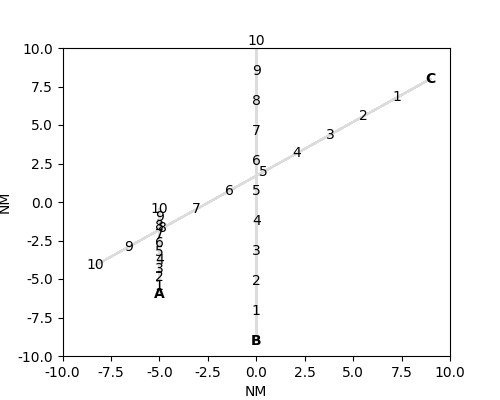
\includegraphics[width=0.75\textwidth,height=0.75\textheight,keepaspectratio]{../src/img/overtaking_crossing.png}
    \caption[Overtaking and crossing scenario 1]{Overtaking and crossing scenario 1 \cite{ecolreg_overtaking-and-crossing}}
    \label{fig:overtaking-and-crossing}
\end{figure}
The three following scenarios all depict scenarios where vessels \textit{A} and \textit{B} are in an overtaking situation while \textit{C} crosses both their paths. \textit{C} crosses \textit{A} and \textit{B}s paths with a \ang{45}  angle in the first scenario (figure \ref{fig:overtaking-and-crossing}). \textit{A} starts at (-5, -6), \textit{B} at (0, -9) and \textit{C} in (9, 8). \textit{A} and \textit{B} has an initial heading of \ang{0}  while \textit{C} start with a heading of \ang{235}. The speeds of the vessels is set to ensure that \textit{C} will collide with both vessels if no corrections are applied. Moreover, the speed of \textit{B} must be greater than the speed of \textit{A} since \textit{B} is overtaking \textit{A}. The vessels initial speeds are, therefore: \textit{A} = 2 kts, \textit{B} = 7 kts and \textit{C} = 7.6 kts. The maximum speeds of the vessels are 10, 15 and 20 kts respectively. Maximum rate of turn of all vessels is set to \ang{3} per second.

Rule 13 and 16 apply to this scenario in the same way as the previous one, with the exception that the vessels involved in the overtaking situation is vessel \textit{A} and \textit{B} instead of \textit{B} and \textit{C}. This implies that \textit{B} shall keep out of way of \textit{A} (\textit{Rule 13}), while \textit{A} shall keep its course and speed (\textit{Rule 17}).

Additionally, both \textit{A} and \textit{B} are crossing \textit{C}s path with a risk of collision. This means that \textit{A} and \textit{B} should alter their courses to starboard and avoid passing in front of \textit{C} (\textit{Rule 15}). Vessel \textit{C} shall, meanwhile, keep its course and speed. This results in contradictory obligations for vessel  \textit{A}, where it should keep its course and speed for \textit{B} and simultaneously keep out of the way for vessel \textit{C}.

\textcite{ecolreg_overtaking-and-crossing} suggest the following manoeuvres for vessel \textit{A} and \textit{B} in accordance with the ordinary practice of seamen:
Both vessels might alter course to starboard and, thereby, pass behind vessel \textit{C}. Alternatively vessel \textit{A} may reduce speed or make a \ang{360} turn to port, while vessel \textit{B} reduces speed, makes a \ang{360} to starboard or alters its course to starboard.

\begin{figure}[H]
    \centering
    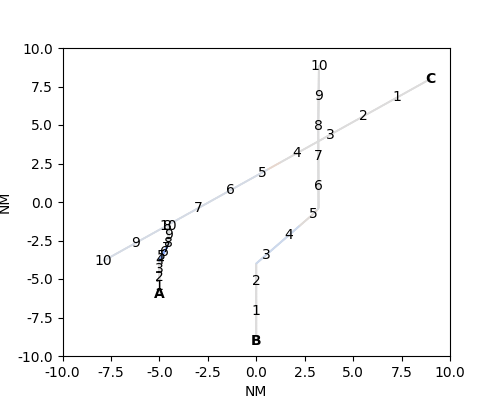
\includegraphics[width=0.75\textwidth,height=0.75\textheight,keepaspectratio]{../src/img/overtaking_crossing_res.png}
    \caption{Overtaking and crossing scenario 1}
    \label{fig:overtaking-and-crossing-res}
\end{figure}

The recommendations by the ANS matches the ordinary practice of seamen quite well for this scenario. Vessel \textit{A} chooses to slow down and alter its course slightly to starboard, while vessel \textit{B} alters its course to starboard. Thus vessel \textit{A} made two corrections instead of one as recommended.  The vessels manage to keep a safe distance and none of the stand on vessels are forced to alter their courses. Vessel \textit{C} keeps its original heading and course during the whole simulation. A visualization can be seen in figure \ref {fig:overtaking-and-crossing-res}.

\section{Overtaking and crossing scenario 2}%----------------------------------------
%------------------------------------------------------------------------------------


\begin{figure}[H]
    \centering
    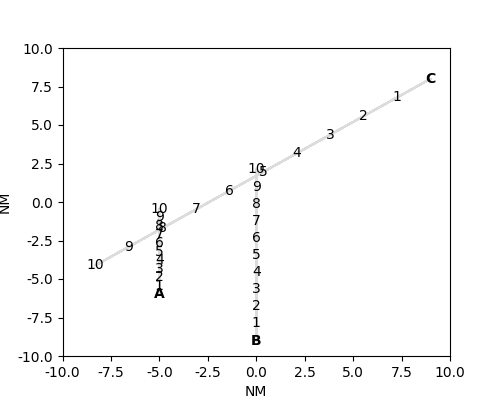
\includegraphics[width=0.75\textwidth,height=0.75\textheight,keepaspectratio]{../src/img/overtaking_crossing_3.png}
    \caption[Overtaking and crossing scenario 2]{Overtaking and crossing scenario 2 \cite{ecolreg_overtaking-and-crossing-3}}
    \label{fig:overtaking-and-crossing-3}
\end{figure}
The next scenario, visualized in figure \ref{fig:overtaking-and-crossing-3}, differs from the previous only in that B and C are not at risk of collision since Bs speed is decreased to 4 kts. This means that B has no obligations to alter its course to starboard to avoid C as in the previous scenario. All other rules from the previous scenario do apply and vessel A is, therefore, still in the contradictory situation where it shall both keep course and speed for vessel B and alter course to starboard to avoid vessel C.

The following actions by vessel A solve the situation in accordance with the ordinary practice of seamen. It might either slow down, make a 360 degree turn to port or alter course to starboard and pass in front of vessel B if time permits.



\begin{figure}[H]
    \centering
    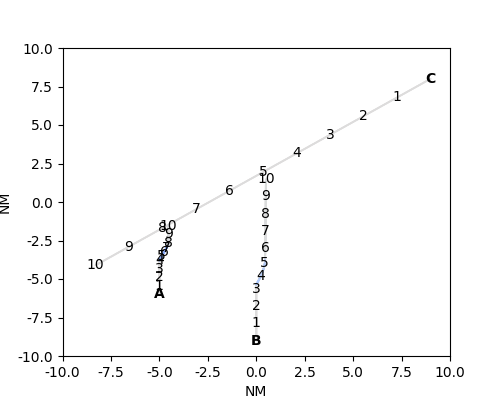
\includegraphics[width=0.75\textwidth,height=0.75\textheight,keepaspectratio]{../src/img/overtaking_crossing_3_res.png}
    \caption{Overtaking and crossing scenario 2}
    \label{fig:overtaking-and-crossing-3-res}
\end{figure}

This scenario is almost identical to the previous with the exception that there is no risk of collision between vessel \textit{B} and \textit{C}. These vessels should therefore, ideally not make any alterations to their courses. However, vessel \textit{A} has to avoid vessel \textit{C}, which is coming from starboard. Figure \ref{fig:overtaking-and-crossing-3-res} shows how vessel \textit{A} both alters course and slows down as in the previous scenario, which causes vessel \textit{B} to also alter its course to starboard to avoid vessel \textit{A}. This manoeuvre by vessel \textit{B} is completely unnecessary since vessel \textit{As} speed is significantly lower than \textit{B's} and a collision is, therefore, not imminent even thought vessel \textit{A} turns towards vessel \textit{B}.

\section{Overtaking and crossing scenario 3}%----------------------------------------
%------------------------------------------------------------------------------------


\begin{figure}[H]
    \centering
    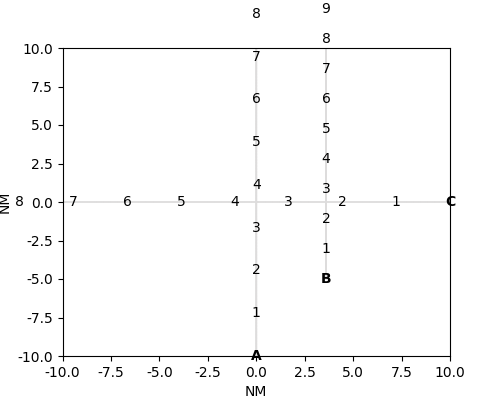
\includegraphics[width=0.75\textwidth,height=0.75\textheight,keepaspectratio]{../src/img/overtaking_crossing_2.png}
    \caption[Overtaking and crossing scenario 3]{Overtaking and crossing scenario 3 \cite{ecolreg_overtaking-and-crossing-2}}
    \label{fig:overtaking-and-crossing-2}
\end{figure}

The last scenario depicts a similar scenario as the previous two, with two vessels in an overtaking situation while a third cross their paths. The scenario is visualized in figure \ref{fig:overtaking-and-crossing-2}. Vessel \textit{A} starts at (0, -10), vessel \textit{B} at (3.6, 5) and \textit{C} at (10, 0). The two vessels involved in the overtaking situation, that is \textit{A} and \textit{B}, start with a heading of \ang{0}  while  \textit{C} starts with a {270} heading in order to cross the two other vessels paths perpendicularly. \textit{A} and \textit{C} start at a speed of 10 kts while \textit{B} starts at 15 kts. All vessels have as maximum speed of 20 kts and a maximum rate of turn of \ang{3} per second. The same rules apply as in the two previous rules, but the manoeuvring space for vessels \textit{A} and \textit{B} is slightly more limited due to the angle which C approaches on.

Vessel \textit{A} is also in this scenario in a situation where two rules contradict each other.
It shall keep course and speed for vessel \textit{B} while simultaneously avoiding vessel \textit{C}.
Vessel \textit{C} shall keep course and speed for both vessel \textit{B} and \textit{A}.
Finally vessel \textit{B} shall keep out of the way of vessel \textit{A} and alter course to starboard to avoid vessel C.

One of the following actions is recommended to avoid collisions \cite{ecolreg_overtaking-and-crossing-2}. Both vessels might alter their course to starboard and pass behind vessel \textit{C} to avoid collision. The action must however be initiated by vessel \textit{B}. Alternatively vessel \textit{A} might either reduce speed or make a 360 degree turn. The turn must be initiated early if made to starboard. Vessel \textit{B} must at the same time also reduce speed, make a \ang{360} turn to starboard or alter course to starboard to avoid colliding with vessel \textit{C}



\begin{figure}[H]
    \centering
    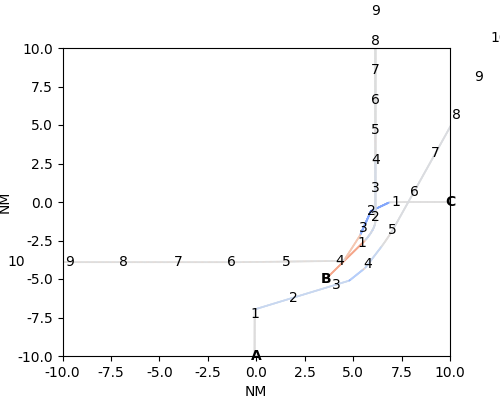
\includegraphics[width=0.75\textwidth,height=0.75\textheight,keepaspectratio]{../src/img/overtaking_crossing_2_res.png}
    \caption{Overtaking and crossing scenario 3}
    \label{fig:overtaking-and-crossing-2-res}
\end{figure}

The ANS simulation starts out as described above with vessels \textit{A} and \textit{B} altering courses to starboard to pass behind vessel \textit{C}. Additionally Vessel A slows down while vessel \textit{B} accelerates. The two vessels avoid each other exactly as described by \textcite{ecolreg_overtaking-and-crossing-2}, apart from the extra speed changes. However, the alterations made by vessel \textit{B} to avoid void vessel \textit{C} and \textit{A} make the distance between vessel \textit{B} and \textit{A} shrink to under $R_b$, which forces vessel \textit{C} to alter its course to port and decrease its speed. This causes vessels \textit{B} to steer towards vessel \textit{C}, thereby increasing the collision risk between the two vessels and breaking the COLREG rules. However, it could be argued that the initial placement of the vessels does not correspond to a normal situation since vessel \textit{B} and \textit{C} start at a distance less than $R_a$ and therefore have limited manoeuvring space.


\chapter{Discussion}%----------------------------------------------------------------
%------------------------------------------------------------------------------------
\label{chap:disc}
The goal of this thesis has been to further examine the work of \textcite{perera2012intelligent}, regarding the use of fuzzy logic to facilitate collision avoidance amongst USVs. The previous research presents successful results in
basic multi vessel situations at sea. However, only one of the vessels featured in the scenarios of that paper uses FIS to navigate. The other vessels
are dummy vessels that keep their speed and course for the whole scenario.
The contribution of this thesis would, therefore, be to test the usage of a FIS
based ANS in scenarios where multiple vessels uses it. Such scenarios put the vessels in situations where they are simultaneously supposed to give way and stand on and thereby has to prioritize the actions suggested by the ANS. An average weighted on expected collision time is used to prioritize the FIS recommended actions, rather
than Bayesian networks, as suggested by \textcite{perera2012intelligent}.

The results of the simulations presented in section \ref{sec:evaluation} show that the FIS based ANS manages to prevent collision in all of the scenarios. Although the corrections made by the vessels were not always in accordance with the ordinary practice of seamen. For instance, the scenarios depicted in figures \ref{fig:overtaking-and-head-on-res} and \ref{fig:overtaking-and-crossing-2-res} show vessels accelerating although the COLREG rules only mention decreasing the speed as a proper response in case of an impending collision. This can to some extent be blamed on the configuration of the FIS, i.e the  antecedents and consequents, as well as the rules, specified. The previously mentioned example stems from a rule with acceleration as a consequent.  The FIS configuration is in other words crucial to the quality of the ANS system. 

The possibility to simply define rules was one of the reasons why fuzzy logic was initially chosen for this thesis since such a system would enable people with navigation expertise to verify the rules even though they do not understand the underlying technology. This would potentially facilitate the process to certify the algorithm as safe. However, a large rule-set  and multiple inputs might quickly become difficult to comprehend since the change in one rule might have implications on how another vessel acts in  certain scenarios. This situations is further complicated by the fact that the parameters would have to be adjusted to suit the particular vessel type the ANS system is a part of. Additionally different rule sets would probably have to be designed for different situations. The scenarios in this thesis are all set on the open sea, while many of the COLREG rules specify more specific situations. This could result in quite large rule-sets, that might be tedious to verify and maintain.

Another issue that needs to be considered is the way the current system defines visible target vessels. This becomes particularly evident in figure \ref{fig:overtaking-and-crossing}, where vessel \textit{B} reaches vessel \textit{A}'s $R_A$ slightly before vessel \textit{C}. This results in vessel \textit{A} accelerating instead of turning further to the right. This situation could possibly be improved by redesigning the range FMF, so that the membership value increases gradually as the vessels approach each other. The current FMF goes from zero to one as the target vessel passes $R_A$. Increasing the fuzzy area of the FMF past $R_A$ with a gradual decrease towards zero could potentially increase the vessels SA, thereby enabling it to make better decisions.

Furthermore, some of the corrections suggested by the ANS could be considered unnecessary. For instance vessel \textit{B's} course change in figure \ref{fig:overtaking-and-crossing-3-res}. COLREGs \textit{rule 7} state that a collision is imminent when two vessels have constant compass bearing over a prolonged time, which is not the case in figure \ref{fig:overtaking-and-crossing-3-res}. The current system lacks this kind of comparison between the  current situation and a previous instance and is therefore, unable to comply with \textit{7}. This might lead to unnecessary corrections and could potentially trigger chain reactions between USV's in range of each other.


\chapter{Conclusions}%---------------------------------------------------------------
\label{chap:conc}

Successful development of USVs able to safely navigate among both other USV and ordinary manned vessels could, apart from being safer,  decrease the operational costs of the maritime shipping industry significantly. However, collision avoidance systems for USVs can be implemented in a variety of ways. The purpose of this thesis has been to evaluate the FIS based collision avoidance algorithm presented by \textcite{perera2012intelligent,perera2010smooth_param}, by reimplementing it in python and increasing the complexity of the tested simulation scenarios. Furthermore, an analysis of the COLREG rules and the fuzzy logic elements used in the algorithm was made in order to reimplement the algorithm and  develop a simulation framework.

Both the research by \textcite{perera2012intelligent,perera2010smooth_param}  and this thesis prove that the developed FIS based ANS do manage to avoid collision between USVs in basic COLREG situations. However, the more complicated scenarios  reveal a few limitations in the algorithm. The decisions made by the algorithm will, for instance, not always follow ordinary practice of seamen and could therefore confuse the crew of manned vessels. Mostly due to the fact that the current implementation  only analyse the present situation and is therefore unable to make decisions based on comparison to previous states.

An initially appealing aspect of the fuzzy logic based solution was the ability to write the navigation logic as IF-THEN based rules, thereby facilitating verification of the algorithm by people not familiar with the underlying logic. However, designing a maintainable and efficient  rule-set could prove complicated. For instance, most of the non COLREGs compliant corrections suggested during the simulations stem from poorly defined rules.





%------------------------------------------------------------------------------------
% Works but might not be the most effecient
% Intheory easy to verify rules

\section{Further work}%--------------------------------------------------------------
%------------------------------------------------------------------------------------
The two major limitations found during the evaluation are, as stated in the previous section, the rule-set and the algorithms inability to make decisions based on a holistic model of the situation.
Further analysis of the rule-set and its corresponding antecedents and consequents is, therefore, needed to ensure safe decisions in all situations. Moreover, improvements should be considered to ensure that the decisions made by the ANS follows ordinary practice of seamen. This improvement includes both rule changes as well as an upgrade to the way multi target situations are prioritized.
Finally system needs to be incorporated into a full ANS with real SA and navigation modules for further testing and simulations.
% Improve rules
% Add way to compare time frames
%Different vessels (fishing, tow, mm)
